En este capítulo se explicará el funcionamiento de la aplicación desde el punto
de vista del usuario final, detallando las opciones de cada una de las secciones.

Para poder acceder a la aplicación, tal y como se explicó en el
\textit{\nameref{sec:mainstalacion}}, será necesario utilizar el comando:

\begin{minted}{bash}
  ./oflute
\end{minted}

\section{Ejecución inicial}
Al lanzar la aplicación, se abrirá una ventana y aparecerán, consecutivamente,
la pantalla de créditos del autor y la pantalla de presentación del
juego. Pasados unos momentos éstas desaparecerán, aunque tiene la opción de
omitir cada una de las pantallas pulsando la tecla \texttt{escape}.

\begin{figure}[h!]
  \centering
  
\includegraphics[width=0.8\textwidth]{apendice_manual_usuario/imagen_estadoAutor}
  \caption{Pantalla de créditos del autor}
  \vspace{-1cm}
\end{figure}

\begin{figure}[h!]
  \centering
  
\includegraphics[width=0.8\textwidth]{apendice_manual_usuario/imagen_estadoIntro}
  \caption{Pantalla de presentación del juego}
  \vspace{-0.3cm}
\end{figure}

Una vez desaparezcan ambas pantallas, se iniciará una animación para mostrar el
menú principal. Puede cancelar la animación y mostrar rápidamente el menú
principal pulsando la tecla \texttt{escape}.

\begin{figure}[h!]
  \centering
  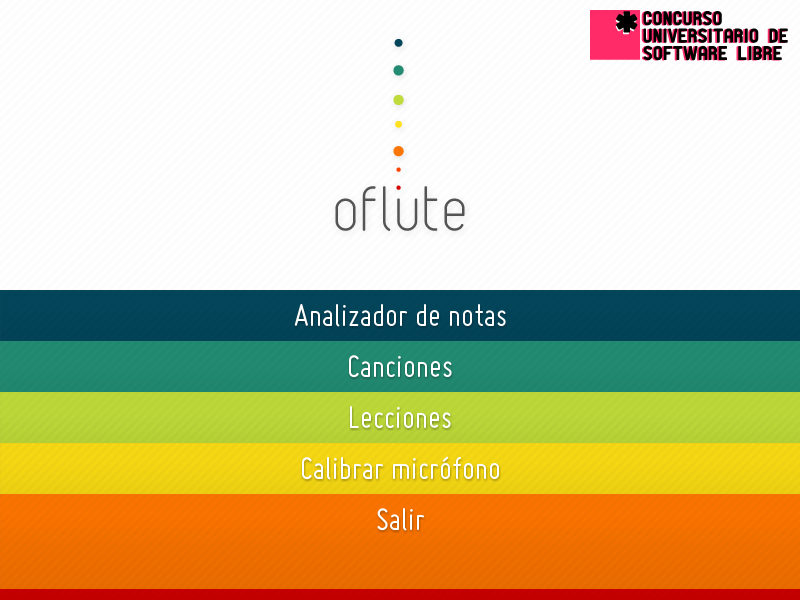
\includegraphics[width=0.8\textwidth]{apendice_manual_usuario/imagen_menuPrincipal}
  \caption{Pantalla del menú principal}
  \vspace{-1cm}
\end{figure}




